\section{eo\-Timed\-Dyn\-Update Class Reference}
\label{classeo_timed_dyn_update}\index{eoTimedDynUpdate@{eoTimedDynUpdate}}
An {\bf eo\-Updater}{\rm (p.\,\pageref{classeo_updater})} to update an {\bf eo\-Updatable}{\rm (p.\,\pageref{classeo_updatable})} object every given time interval.  


{\tt \#include $<$eo\-Updatable.h$>$}

Inheritance diagram for eo\-Timed\-Dyn\-Update::\begin{figure}[H]
\begin{center}
\leavevmode
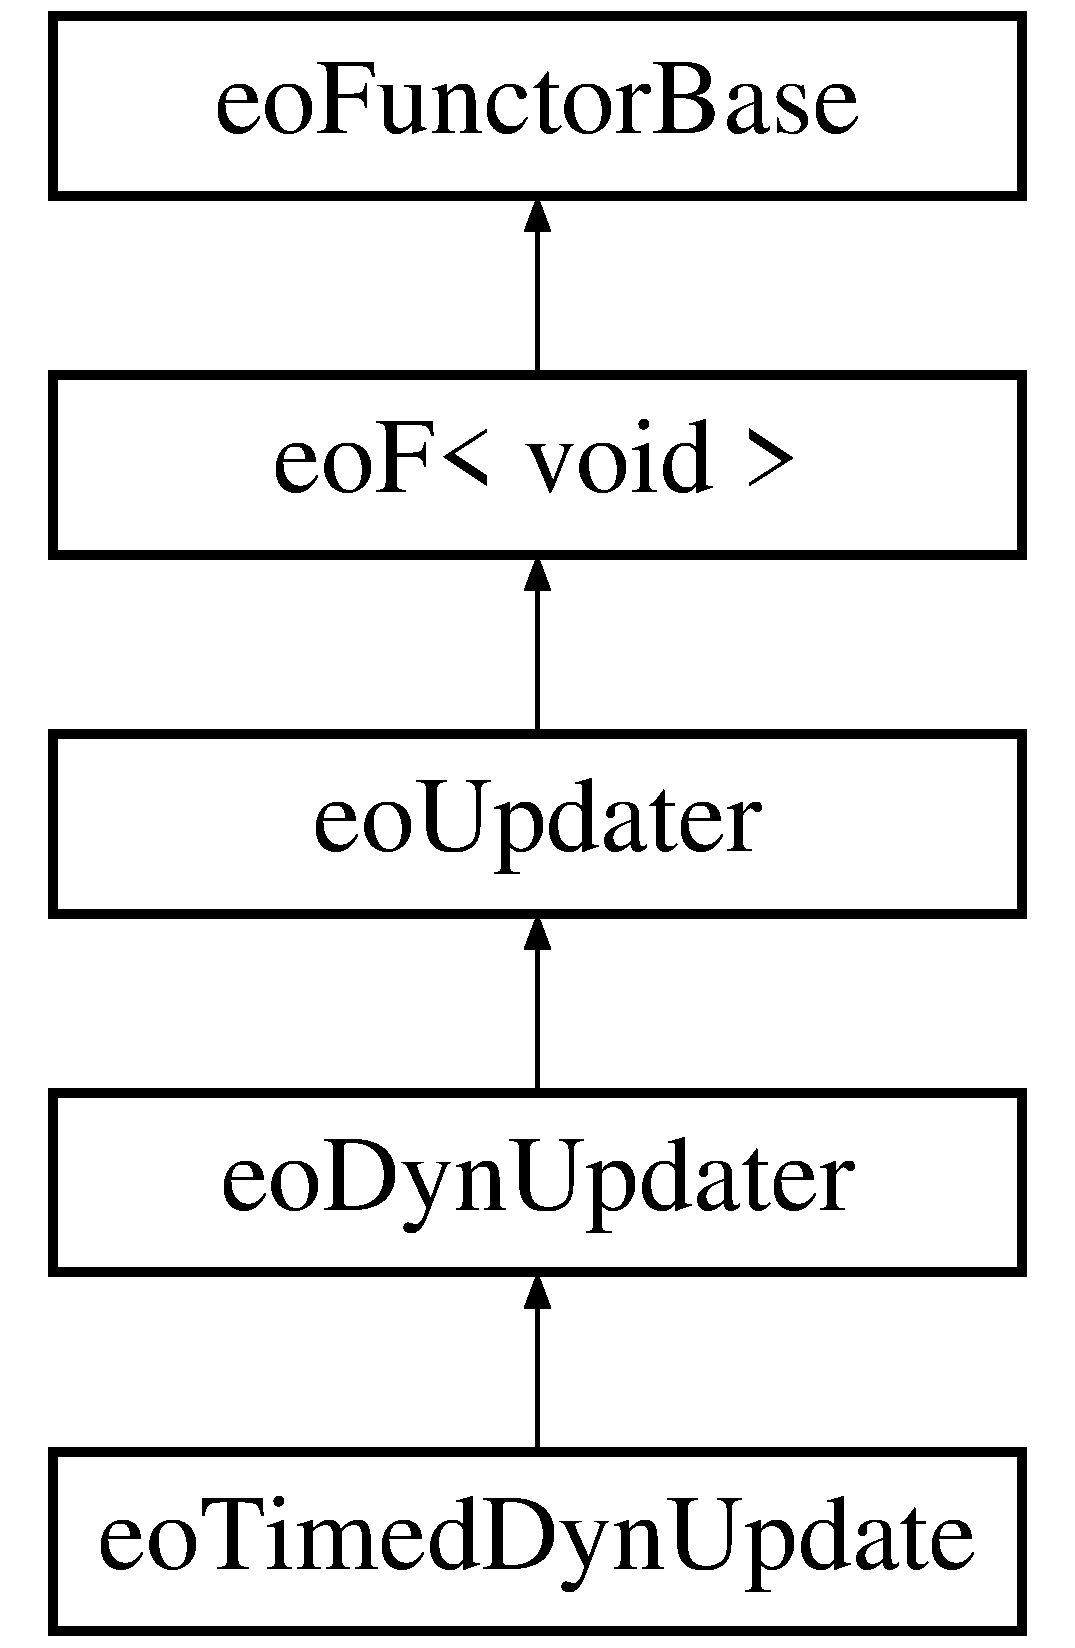
\includegraphics[height=5cm]{classeo_timed_dyn_update}
\end{center}
\end{figure}
\subsection*{Public Member Functions}
\begin{CompactItemize}
\item 
{\bf eo\-Timed\-Dyn\-Update} ({\bf eo\-Updatable} \&\_\-to\-Update, time\_\-t \_\-interval)\label{classeo_timed_dyn_update_a0}

\item 
void {\bf operator()} (void)\label{classeo_timed_dyn_update_a1}

\begin{CompactList}\small\item\em The pure virtual function that needs to be implemented by the subclass. \item\end{CompactList}\end{CompactItemize}
\subsection*{Private Attributes}
\begin{CompactItemize}
\item 
const time\_\-t {\bf interval}\label{classeo_timed_dyn_update_r0}

\item 
time\_\-t {\bf last\_\-time}\label{classeo_timed_dyn_update_r1}

\item 
const time\_\-t {\bf first\_\-time}\label{classeo_timed_dyn_update_r2}

\end{CompactItemize}


\subsection{Detailed Description}
An {\bf eo\-Updater}{\rm (p.\,\pageref{classeo_updater})} to update an {\bf eo\-Updatable}{\rm (p.\,\pageref{classeo_updatable})} object every given time interval. 



Definition at line 67 of file eo\-Updatable.h.

The documentation for this class was generated from the following file:\begin{CompactItemize}
\item 
eo\-Updatable.h\end{CompactItemize}
